\documentclass[a4paper, 12pt]{scrartcl}

\usepackage[dvipsnames, svgnames, table]{xcolor}

\usepackage{amsmath, amssymb}
\usepackage{ntheorem}
\usepackage{enumitem}

\usepackage{multicol,paracol}

\usepackage{pgfplots}
\pgfplotsset{compat=1.15}
\usepackage{mathrsfs}
\usetikzlibrary{arrows}

\usepackage{graphicx}
\usepackage{float}
\graphicspath{{imagini}, {grafice}}


\theoremstyle{plain}
\newtheorem{subiect}{Subiectul}

\newcommand{\Subiect}[1]{
    {
        \large
        \begin{subiect}
            #1
        \end{subiect}
    }
}

\title{
    Test de evaluare
}
\subtitle{Func\c tii \c si ecua\c tii \\
exponen\c tiale \c si logaritmice}
\author{}
\date{}

\titlehead{
    \footnotesize
    \begin{minipage}[c]{0.10\linewidth}
        
\includegraphics[width=\textwidth]{sigla.png}
    \end{minipage} 
    \begin{minipage}[c]{0.7\linewidth}
        {\small\bfseries Liceul Teoretic ``Alexandru Ioan Cuza'', Iași} \\
        Anul 2022--2023\\
        Matematic\u a-informatic\u a\\
        Clasa a X-a A
    \end{minipage}
}

\begin{document}
\maketitle

\begin{tabular}{l l}
    (*)   & Dificultate redus\u a \hfill \\
    (**)  & Dificultate medie  \\
    (***) & Dificultate ridicat\u a \\
\end{tabular} \\
\indent Timp de lucru: 90 de minute \\
\indent Se acord\u a 2 puncte din oficiu \\

\Subiect{\^ Incercui\c ti r\u aspunsul corect: \hfill (*)}

\begin{description}
    \item[1)] Ecua\c tia \(2 \cdot 3^x = 54 \) are solu\c tia unic\u a: \hfill 1pct
    {
        \begin{paracol}{3}
            \begin{description}
                \item[a.] x = 3 
                \item[b.] x = 2 
            \end{description}
            \switchcolumn
            \begin{description}
                \item[c.] x = 5
                \item[d.] nu are solu\c tie 
            \end{description}
            \switchcolumn
        \end{paracol}
    }
    \item[2)] Ecua\c tia \(5 \cdot \log_2{x} = 640 \) are solu\c tia unic\u a: \hfill 1pct
    {
        \begin{paracol}{3}
            \begin{description}
                \item[a.] x = 3 
                \item[b.] x = 6 
            \end{description}
            \switchcolumn
            \begin{description}
                \item[c.] x = 7
                \item[d.]nu are solu\c tie 
            \end{description}
            \switchcolumn
        \end{paracol}
    }
\end{description}

\newpage

\Subiect{(Varianta I) Uni\c ti fiecare func\c tie cu graficul corespunz\u ator: (4 \(\cdot\) 0.5pct) \hfill (*)}

\begin{paracol}{2}
    \noindent
    1. \( f: \mathbb{R} \rightarrow ( 0, \infty ),  f(x) = 2^x \)
    \switchcolumn
    {
        \definecolor{qqwuqq}{rgb}{0,0.39215686274509803,0}
        \begin{tikzpicture}[line cap=round,line join=round,>=triangle 45,x=1cm,y=1cm]
        \begin{axis}[
        x=0.7cm,y=0.7cm,
        axis lines=middle,
        ymajorgrids=true,
        xmajorgrids=true,
        xmin=-4.1802214080407145,
        xmax=4.334707151719486,
        ymin=-1.0068709262965196,
        ymax=4.0072855294173895,
        xtick={-4,-3,...,4},
        ytick={0,1,...,3},]
        \clip(-4.1802214080407145,-1.0068709262965196) rectangle (4.334707151719486,4.0072855294173895);
        \draw[line width=2pt,color=qqwuqq,smooth,samples=100,domain=-4.1802214080407145:4.334707151719486] plot(\x,{2^((\x))});
        \begin{scriptsize}
        \draw[color=qqwuqq] (-4.111690795889726,0.12673961636772973) node {$f$};
        \end{scriptsize}
        \end{axis}
        \end{tikzpicture}
    }
\end{paracol}

\begin{paracol}{2}
    \noindent
    2. \( f: ( 0, \infty ) \rightarrow \mathbb{R}, f(x) = \log_2{x} \)
    \switchcolumn
    {
        \definecolor{qqwuqq}{rgb}{0,0.39215686274509803,0}
        \begin{tikzpicture}[line cap=round,line join=round,>=triangle 45,x=1cm,y=1cm]
        \begin{axis}[
        x=0.7cm,y=0.7cm,
        axis lines=middle,
        ymajorgrids=true,
        xmajorgrids=true,
        xmin=-4.1802214080407145,
        xmax=4.1802214080407145,
        ymin=-4.012180415312024,
        ymax=2.0072855294173895,
        xtick={-6,-5,...,7},
        ytick={-4,-3,...,4},]
        \clip(-7.435933582696904,-4.012180415312024) rectangle (7.667561913196296,4.881762606414469);
        \draw[line width=2pt,color=qqwuqq,smooth,samples=100,domain=1.0000001289061244:7.667561913196296] plot(\x,{ln((\x)-1)/ln(2)});
        \begin{scriptsize}
        \draw[color=qqwuqq] (1.1034672912386876,-3.8146497901142253) node {$f$};
        \end{scriptsize}
        \end{axis}
        \end{tikzpicture}
    }
\end{paracol}
    
\begin{paracol}{2}
    \noindent
    3. \( f: \mathbb{R} \rightarrow ( 0, \infty ), f(x) = 2^{x+1} - 1 \)
    \switchcolumn
    {
        \definecolor{qqwuqq}{rgb}{0,0.39215686274509803,0}
        \begin{tikzpicture}[line cap=round,line join=round,>=triangle 45,x=1cm,y=1cm]
        \begin{axis}[
        x=0.7cm,y=0.7cm,
        axis lines=middle,
        ymajorgrids=true,
        xmajorgrids=true,
        xmin=-4.189591779594589,
        xmax=4.161111482398531,
        ymin=-2.4893889458473266,
        ymax=2.428060728217025,
        xtick={-4,-3,...,4},
        ytick={-2,-1,...,2},]
        \clip(-4.189591779594589,-2.4893889458473266) rectangle (4.161111482398531,2.428060728217025);
        \draw[line width=2pt,color=qqwuqq,smooth,samples=100,domain=0.000006151166931241844:4.161111482398531] plot(\x,{ln((\x))/ln(2)});
        \begin{scriptsize}
        \draw[color=qqwuqq] (0.20138833938770914,-2.3801745168675374) node {$f$};
        \end{scriptsize}
        \end{axis}
        \end{tikzpicture}
    }
\end{paracol}

\begin{paracol}{2}
    \noindent
    4. \( f: \mathbb{R} \rightarrow ( 0, \infty ), f(x) = \log_2({x - 1}) \)
    \switchcolumn
    {
        \definecolor{qqwuqq}{rgb}{0,0.39215686274509803,0}
        \begin{tikzpicture}[line cap=round,line join=round,>=triangle 45,x=1cm,y=1cm]
        \begin{axis}[
        x=0.7cm,y=0.7cm,
        axis lines=middle,
        ymajorgrids=true,
        xmajorgrids=true,
        xmin=-4.189591779594589,
        xmax=4.161111482398531,
        ymin=-2.4893889458473266,
        ymax=2.428060728217025,
        xtick={-4,-3,...,4},
        ytick={-2,-1,...,2},]
        \clip(-6.927933621789031,-3.55147637691946) rectangle (6.802516829022966,4.533926370104626);
        \draw[line width=2pt,color=qqwuqq,smooth,samples=100,domain=-4.189591779594589:4.189591779594589] plot(\x,{2^((\x)+1)-1});
        \begin{scriptsize}
        \draw[color=qqwuqq] (-6.817426978321731,-0.8762947163152496) node {$f$};
        \end{scriptsize}
        \end{axis}
        \end{tikzpicture}
    }
\end{paracol}

\newpage
\noindent (Varianta II) Uni\c ti fiecare func\c tie cu graficul corespunz\u ator: (4 \(\cdot\) 0.5pct) \hfill (*)


\begin{paracol}{2}
    \noindent
    1. \( f: \mathbb{R} \rightarrow ( 0, \infty ),  f(x) = 2^x \)
    \switchcolumn
    \begin{figure}
        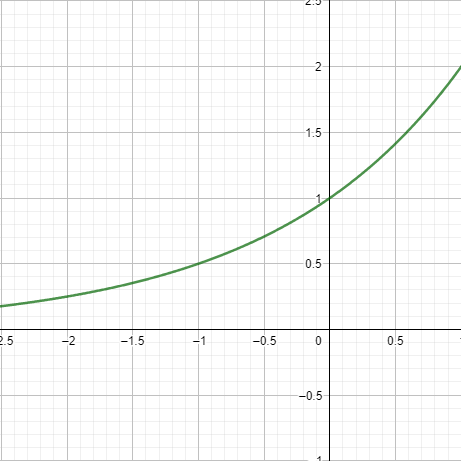
\includegraphics[width=0.27\textwidth]{g1.png}
    \end{figure}
\end{paracol}

\begin{paracol}{2}
    \noindent
    2. \( f: ( 0, \infty ) \rightarrow \mathbb{R}, f(x) = \log_2{x} \)
    \switchcolumn
    \begin{figure}
        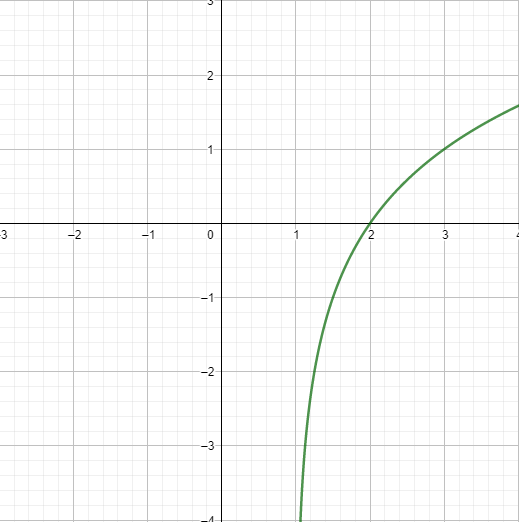
\includegraphics[width=0.27\textwidth]{g2.png}
    \end{figure}
\end{paracol}
    
\begin{paracol}{2}
    \noindent
    3. \( f: \mathbb{R} \rightarrow ( 0, \infty ), f(x) = 2^{x+1} - 1 \)
    \switchcolumn
    \begin{figure}
        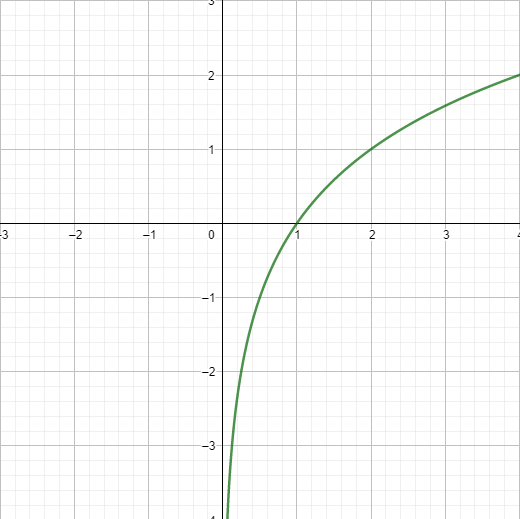
\includegraphics[width=0.27\textwidth]{g3.png}
    \end{figure}
\end{paracol}

\begin{paracol}{2}
    \noindent
    4. \( f: \mathbb{R} \rightarrow ( 0, \infty ), f(x) = \log_2({x - 1}) \)
    \switchcolumn
    \begin{figure}[h]
        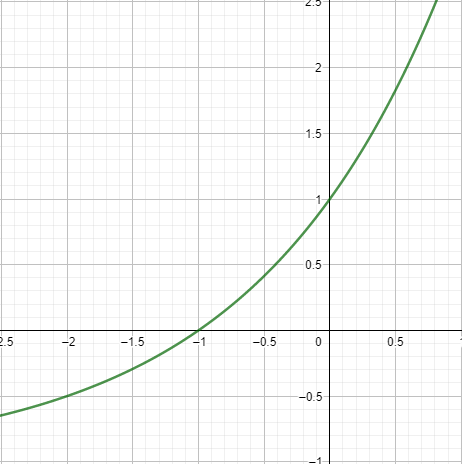
\includegraphics[width=0.27\textwidth]{g4.png}
    \end{figure}
\end{paracol}

\newpage

\Subiect{Rezolva\c ti complet urm\u atoarele exerci\c tii:}

\begin{enumerate}[label=\textbf{\arabic*})]
    \item {
        Rezolva\c ti \^in mul\c timea numerelor reale urm\u atoarea ecua\c tie exponen\c tial\u a: (**) \hfill (1pct)
        \[
            4^x - 3 \cdot 2^x + 2 = 0
        \]    
    }
    \item {
        Rezolva\c ti \^in mul\c timea numerelor reale urm\u atoarea ecua\c tie logaritmic\u a: (**) \hfill (1pct)
        \[
            \log_2 (x^2 - x - 2) - \log_2 (2x - 4) = 1
        \]    
    }
\end{enumerate}

\Subiect{Rezolva\c ti complet urm\u atoarele exerci\c tii:}
\begin{enumerate}[label=\textbf{\arabic*})]
    \item {
        S\u a se determine valorile pozitive ale num\u arului \(x\) \c stiind c\u a \( \lg \sqrt{x}, \frac{3}{2} \) \c 
        si \( \lg x \) sunt termenii consecutivi ai unei progresii aritmetice: (***) \hfill (1pct)
    }
    \item {
        Rezolva\c ti urm\u atoarea ecua\c tie exponen\c tial\u a: (***) \hfill (1pct)
        \[
            2^x + 3^x = 2 \cdot 5^x    
        \]    
        \textit{Indica\c tie:} Dac\u a \( f:D \subset \mathbb{R} \rightarrow \mathbb{R} \) e o func\c tie strict monoton\u a pe D,
        atunci ecua\c tia: \( f(x) = y \) are cel mult o solu\c tie \( \forall y \in \mathbb{R} \) 
    }
\end{enumerate}

\end{document}